
% part 13
\section{Deferred'ы из Deferred'ов\label{sec:part13}}

\subsection{Введение}


Вспомним поэтический клиент 5.1 из главы 10. Он 
использовал Deferred для управления цепочкой callback'ов, 
в которую было включено обращение к поэтическому 
трансформирующему движку. В клиенте 5.1, движок 
релизован как синхронный вызов фукнкции, реализованный в 
самом клиенте.


Теперь мы хотим сделать новый клиент, который 
использует сетевой сервис преобразования поэзии 
из главы \ref{sec:part12}. Здесь есть один ньюанс: 
поскольку трансформирующий сервер доступен по сети, то 
нам нужно будет использовать асинхронный ввод-вывод. И  
это означает, что наш API, запрашивающий трансформацию,  
должен быть асинхронным. Другими словами, callback 
try\_to\_cummingsify в нашем клиенте будет возвращать Deferred. 


Что происходит, когда callback в цепочке deferred'а 
возвращает другой deferred? Давайте назовем первый 
deferred ``внешним'' deferred'м, а второй - ``внутренним''. 
Предположим, что N-ый callback во внешнем deferred'е 
возвратил внутренний deferred. Этот callback говорит: 
``Я асинхронный, моего результата еще здесь нет''. 
Поскольку внешнему deferred'у нужно вызывать следующий  
callback или errback в цепочке с результатом, то 
внешнему deferred'у придется ждать активизации 
внутреннего deferred'а. Конечно же, внешний deferred 
не может блокировать,   
так что вместо этого он приостанавливает 
выполнение цепочки callback и возвращает управление 
реактору (или тому, кто его активизировал).


И каким образом внешний deferred узнает, когда возобновиться? 
Просто - путем добавления пары callback/errback во внутренний 
deferred. Таким образом, когда внутренний deferred 
активизируется, для внешнего deferred'а выполнение его цепочки 
будет возобновлено. Если внутренний deferred успешно завершается (например, 
он вызвал callback, добавленный внешним deferred'ом), то 
внешний deferred вызывает свой N+1'ый callback с результатом. И если 
внутренний deferred завершился с ошибкой (вызвал errback, добавленный 
внешний deferred'ом), то внешний deferred вызовет N+1'ый errback c failure.   


Это нужно осознать, поэтому давайте проиллюстрируем эту идею 
на рисунке \ref{fig:deferred-11}.

\begin{figure}[h]
\begin{center}
    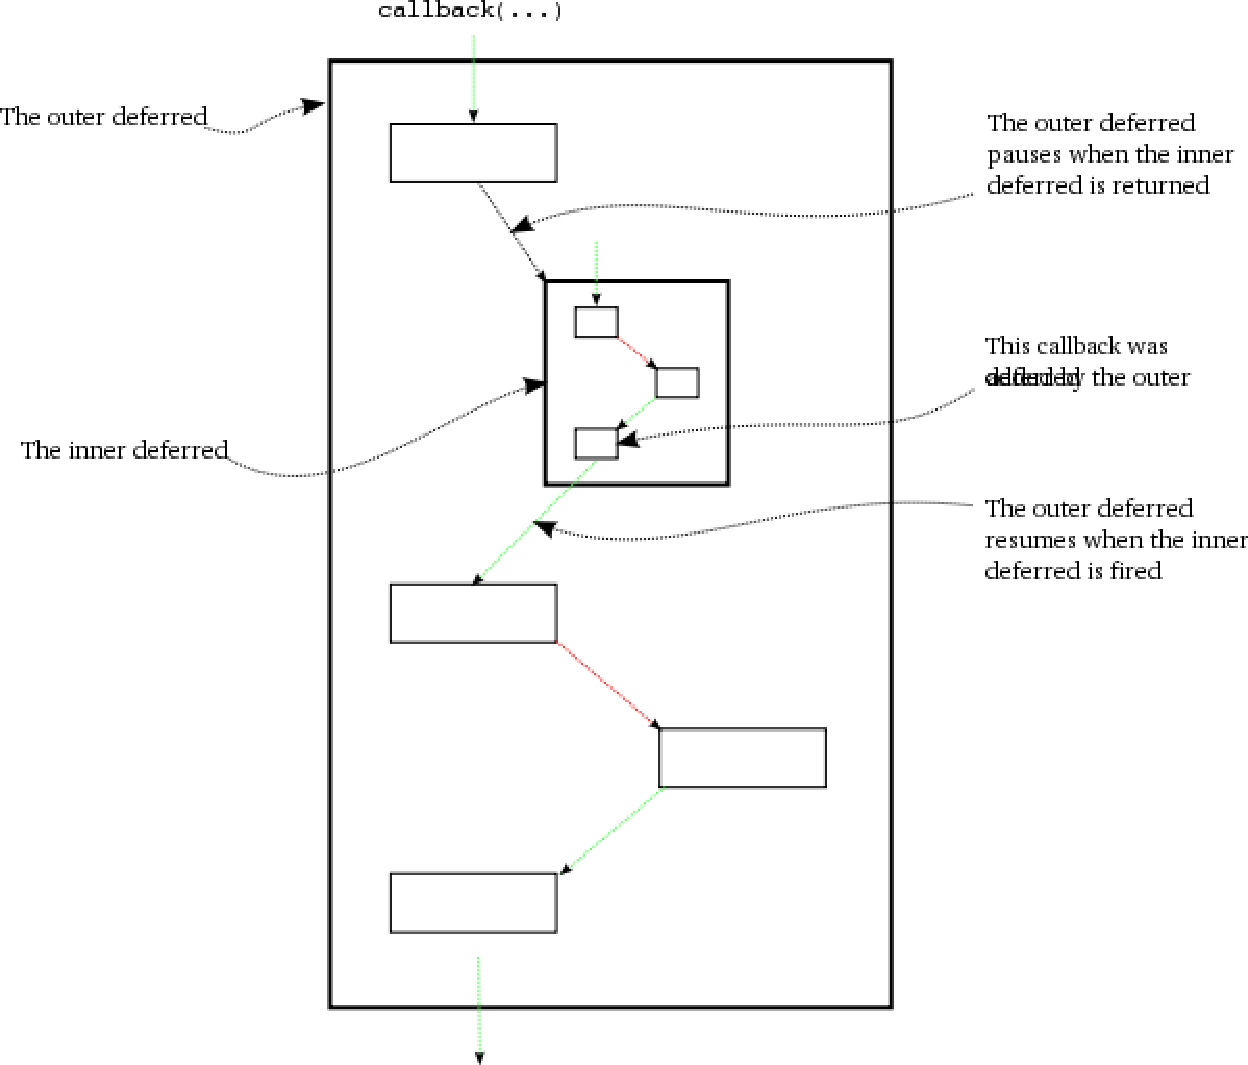
\includegraphics[width=0.8\textwidth]{images/deferred-11.pdf}
    \caption{Обработка внутреннего и внешнего deferred'ов\label{fig:deferred-11}}
\end{center}
\end{figure}

На этом рисунке внешний deferred имеет 4 слоя пар callback/errback. 
Когда внешний deferred активизируется, первый callback в цепочке 
возвращает deferred (внутренний). С этого места, внешний deferred 
остановит активизацию своей цепочки и возвратит управление реактору 
(после добавления пары callback/errback во внутренний deferred). 
Затем, через некоторое время, внутренний deferred активизирует 
внешний deferred, и он возобновит обработку своей callback цепочки. 
Заметим, что внешний deferred сам не активизирует внутренний deferred. 
Это было бы невозможно, поскольку внешний deferred не знает, когда 
доступен результат для внутреннего deferred'а, или какой результат для него  
мог бы быть. Вместо этого, внешний deferred просто ожидает (асинхронно) 
активизации внутреннего deferred'а.


Заметим, что линия, соединяющая callback и 
внутренний deferred на рисунке \ref{fig:deferred-11} 
черная, а не зеленая или красная.  Это потому, что мы 
не знаем до того момента как внутренний deferred не активизируется
был ли этот callback успешно выполнен, или он был выполнен 
с ошибками.  


На рисунке \ref{fig:deferred-12} показана та же последовательность 
внутренних и внешних deferred'в, что и на рисунке \ref{fig:deferred-11}, 
с точки зрения реактора.

\begin{figure}[h]
\begin{center}
    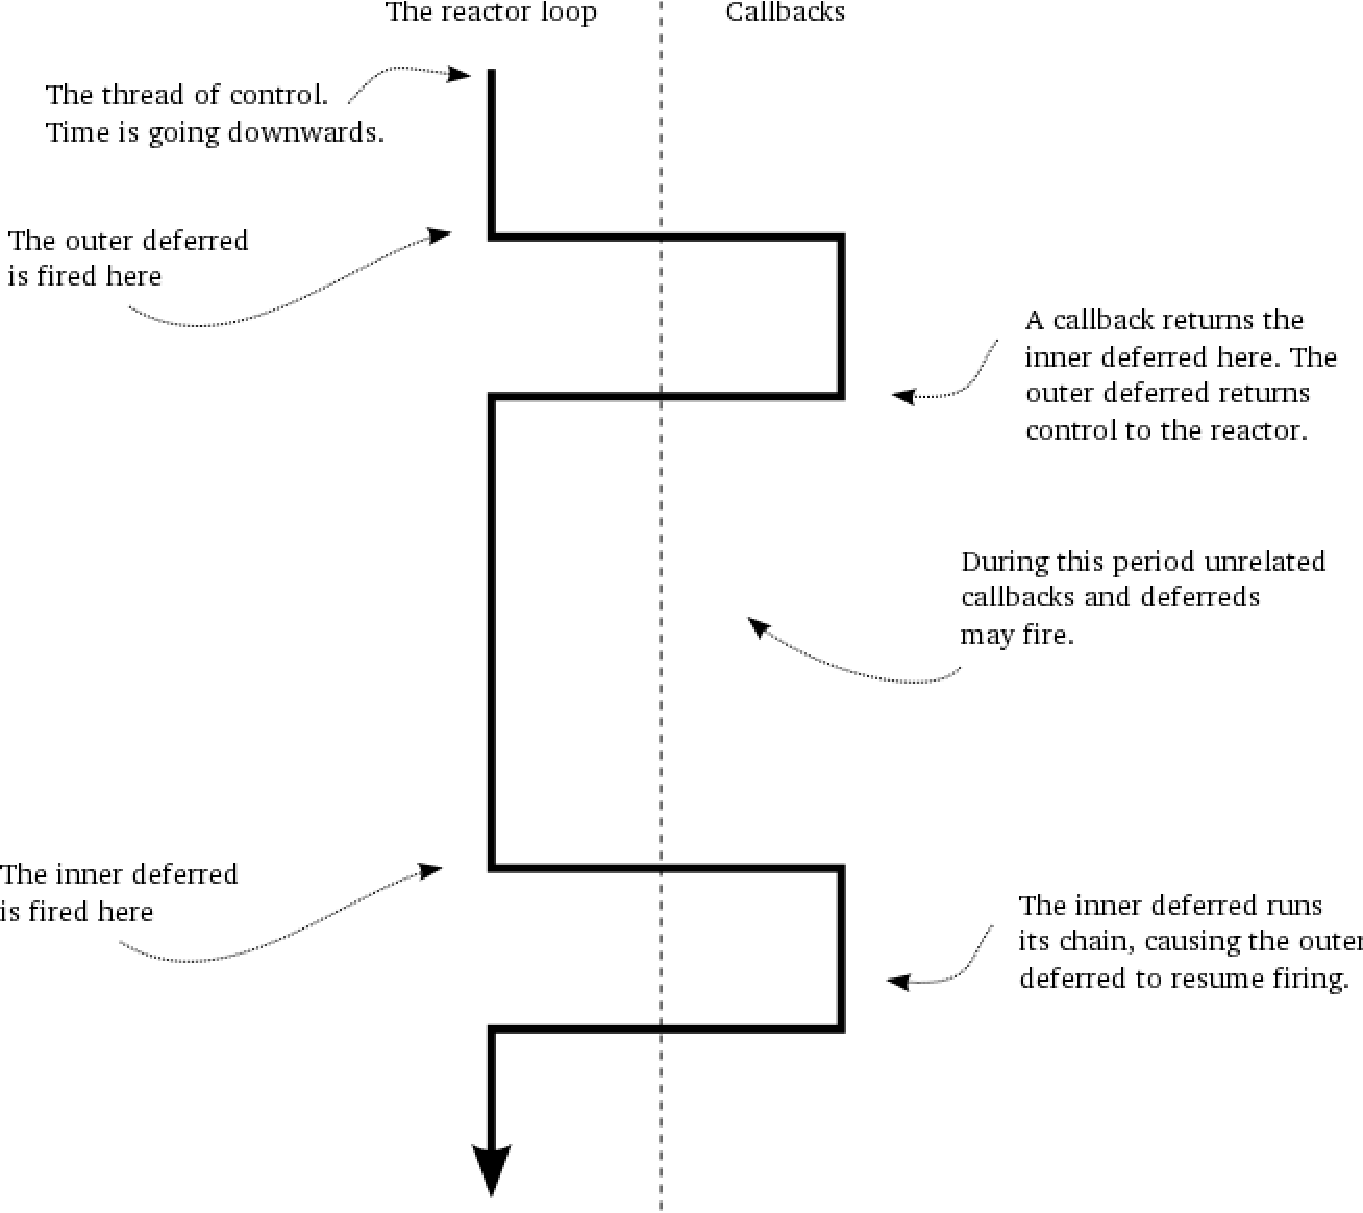
\includegraphics[width=0.8\textwidth]{images/deferred-12.pdf}
    \caption{Поток выполнения при обработке внутренних и внешних deferred'в\label{fig:deferred-12}}
\end{center}
\end{figure}

Это вероятно самое сложное свойство класса Deffered, 
поэтому не беспокойтесь, если вам нужно некоторое время, 
что бы понять. Мы проиллюстрируем это еще одним способом, 
используя пример кода из 
\href{http://github.com/jdavisp3/twisted-intro/blob/master/twisted-deferred/defer-10.py#L1}{twisted-deferred/defer-10.py}. Этот пример создает два внешних deferred'а: 
один - с обычными callback'ми, другой - с callback'ми, один из которых 
возвращает внутренний deferred. Изучая код, и то, что он выводит, 
вы можете увидеть, как второй, внешний, deferred останавливает 
выполнение своей цепочки в момент, когда внутренний  
deferred возвращается,  и после этого возобновляет выполнение, когда 
внутренний deferred активизирован.


\subsection{Клиент 6.0}


Давайте использовать наше новое знание о вложенных 
deferred'х и реализуем заново наш поэтический клиент для 
использования сетевого трансформирующего сервиса из 
главы 12. Вы можете найти его код в 
\href{http://github.com/jdavisp3/twisted-intro/blob/master/twisted-client-6/get-poetry.py#L1}{twisted-client-6/get-poetry.py}. Поэтические Protocol и Factory не 
изменялись и остались такими же как и в предыдущей версии. 
Но теперь появились новые Protocol и Factory для создания запросов 
на преобразование. Далее 
\href{http://github.com/jdavisp3/twisted-intro/blob/master/twisted-client-6/get-poetry.py#L85}{Protocol} 
трансформирующего клиента:

\begin{scriptsize}\begin{verbatim} 
class TransformClientProtocol(NetstringReceiver):

    def connectionMade(self):
        self.sendRequest(self.factory.xform_name, self.factory.poem)

    def sendRequest(self, xform_name, poem):
        self.sendString(xform_name + '.' + poem)

    def stringReceived(self, s):
        self.transport.loseConnection()
        self.poemReceived(s)

    def poemReceived(self, poem):
        self.factory.handlePoem(poem)
\end{verbatim}\end{scriptsize}


Используя NetstringReceiver как базовый класс 
делает реализацию достаточно простой. Как только 
соединение установлено, мы отправляем запрос на 
трансформацию серверу, получая название трансформации 
и поэмы из TransformClientFactory. И, когда мы получаем поэму 
обратно, мы подставляем его в factory для обработки. 
Далее следует код для TransformClientFactory:

\begin{scriptsize}\begin{verbatim}
class TransformClientFactory(ClientFactory):

    protocol = TransformClientProtocol

    def __init__(self, xform_name, poem):
        self.xform_name = xform_name
        self.poem = poem
        self.deferred = defer.Deferred()

    def handlePoem(self, poem):
        d, self.deferred = self.deferred, None
        d.callback(poem)

    def clientConnectionLost(self, _, reason):
        if self.deferred is not None:
            d, self.deferred = self.deferred, None
            d.errback(reason)

    clientConnectionFailed = clientConnectionLost
\end{verbatim}\end{scriptsize}


Эта factory спроектирована для клиентов и управляет 
одним запросом на трансформацию, сохраняя название 
трансформации и поэму для использования Protocol'ом. 
Factory создает единственный Deferred, 
который представляет результат трансформирующего заспроса. 
Заметим, что TransformClientFactory управляет двумя случаями ошибок: 
ошибка соединения и соединение, разорванное в процессе 
получения поэмы. Также нужно отметить, что метод clientConnectionLost 
вызывается даже, если мы получили поэму, и не возникли ошибки, 
но в этом случае self.deferred будет None, благодаря методу handlePoem.


Класс TransformClientFactory создает Deferred, который он также 
активизирует. Хорошее правило следовать такой схеме в 
Twisted программировании, поэтому подчеркнем это:


\hrulefill{
Объекту, который создает Deferred, следует нести 
ответственность за активизацию этого Deferred'а.}


Правила ``ты делаешь - ты и активизируешь'' помогает гарантировать, 
что данный deferred будет активизирован только один раз, и 
улучшает читаемость Twisted программы.


В дополнение к TransformClientFactory, есть также класс 
\href{http://github.com/jdavisp3/twisted-intro/blob/master/twisted-client-6/get-poetry.py#L122}{Proxy}, 
который прячет детали создания TCP соединения к определенному 
трансформирующему сервису:

\begin{scriptsize}\begin{verbatim}
class TransformProxy(object):
    """
    I proxy requests to a transformation service.
    """

    def __init__(self, host, port):
        self.host = host
        self.port = port

    def xform(self, xform_name, poem):
        factory = TransformClientFactory(xform_name, poem)
        from twisted.internet import reactor
        reactor.connectTCP(self.host, self.port, factory)
        return factory.deferred
\end{verbatim}\end{scriptsize}


Этот класс представляет единственный интерфейс xform(), 
который может использоваться для запросов на преобразование. 
Так что в остальном коде можно просто запрашивать трансформацию и 
получать обратно deferred, не заботясь о названиях хостов и 
номерах портов. 


Оставшаяся часть программы не изменилась, за исключением 
\href{http://github.com/jdavisp3/twisted-intro/blob/master/twisted-client-6/get-poetry.py#L163}{try\_to\_cummingsify} callback'а:

\begin{scriptsize}\begin{verbatim}
    def try_to_cummingsify(poem):
        d = proxy.xform('cummingsify', poem)

        def fail(err):
            print >>sys.stderr, 'Cummingsify failed!'
            return poem

        return d.addErrback(fail)
\end{verbatim}\end{scriptsize}


Этот callback теперь возвращает deferred, но 
мы не должны менять 
ничего кроме создания экземпляра Proxy в
оставшейся части функции. 
Поскольку try\_to\_cummingsify был частью цепочки 
deferred'а (возвращаемого get\_poetry), 
то он уже используется асинхронно, и ничего не надо менять. 


Вы заметите, что мы возвращаем результат вызова d.addErrback(fail). 
Это только немного синтаксического сахара. Методы 
addCallback и addErrback возвращают оригинальный deferred. Мы могли 
бы написать двустрочный эквивалент:

\begin{scriptsize}\begin{verbatim}
        d.addErrback(fail)
        return d
\end{verbatim}\end{scriptsize}

\subsection{Тестирование клиента}


Новый клиент имеет немного отличающийся от ранее написанных 
клиентов синтаксис. Если бы вы имели трансформирующий 
сервис, запущенный на порту 10001, и два поэтических сервера, запущенных на 
портах 10002 и 10003, вы бы запустили:

\begin{scriptsize}\begin{verbatim}
python twisted-client-6/get-poetry.py 10001 10002 10003
\end{verbatim}\end{scriptsize}

Для того, чтобы скачать две поэмы и обе их трансформировать, 
вы можете запустить трансформирующий сервер следующим образом:

\begin{scriptsize}\begin{verbatim}
python twisted-server-1/tranformedpoetry.py --port 10001
\end{verbatim}\end{scriptsize}

И поэтические сервера так:

\begin{scriptsize}\begin{verbatim}
python twisted-server-1/fastpoetry.py --port 10002 poetry/fascination.txt
python twisted-server-1/fastpoetry.py --port 10003 poetry/science.txt
\end{verbatim}\end{scriptsize}


%Then you can run the poetry client as above. After that, try crashing the transform server and re-running the client with the same command.

Затем вы можете запустить поэтический клиент как это было 
написано выше. После этого, попробуйте сломать трасформирующий сервер и 
перезапустить клиент той же командой.


\subsection{Резюме}


В этой главе мы изучили то, как deferred'ы могут 
прозрачно управлять другими deferred'ми в callback-цепочке, 
таким образом, мы можем безопасно добавлять асинхронные 
callback'ки во ``внешние'' deferred'ы не заботясь о деталях. 
Это очень удобно, поскольку большинство наших функций, 
в конечном счете, собираются стать асинхронными. 


Знаем ли мы все о deferred'ах? Еще нет! Существует еще 
одна важная особенность, про которую мы поговорим в главе 14.


\subsection{Упражнения}

\begin{enumerate}

\item Модифицируйте клиент так, чтобы мы могли запрашивать определенный 
вид трансформации по названию.

\item Модифицируйте клиент так, чтобы адрес преобразующего сервера 
являлся необязательным аргументом. Если он не задан, то пропускать стадию 
преобразования.

\item Сейчас \href{http://github.com/jdavisp3/twisted-intro/blob/master/twisted-client-6/get-poetry.py#L67}{PoetryClientFactory} 
нарушает правило для deferred'ов  
``ты создавал - ты и активизируй''. Улучшите get\_poetry и 
PoetryClientFactory для того, чтобы это вылечить.

\item Хотя, мы это не демонстрировали, но случай, когда errback возвращает 
deferred является симметричным. Поменяйте пример 
\href{http://github.com/jdavisp3/twisted-intro/blob/master/twisted-deferred/defer-10.py#L1}{twisted-deferred/defer-10.py}, чтобы это проверить.

\item Найдите место в реализации Deferred, которое управляет 
случаем, когда callback/errback возвращает еще один Deferred.

\end{enumerate}


